\documentclass{article}
\usepackage{polski}
\usepackage{graphicx}
\usepackage{amsmath}
\usepackage{hyperref}
\usepackage{float}
\graphicspath{ {./img/} }

\title{Sprawozdanie 1 - Wprowadzenie do Sztucznej Inteligencji}
\author{Michał Kallas}

\begin{document}

\maketitle

\section{Zadanie 1}
\subsection{Polecenie}
Korzystając z jednej z dostępnych bibliotek (np. Keras/TensorFlow, PyTorch, czy scikit-
learn) stwórz i wytrenuj sieć neuronową rozpoznającą cyfry z podanego zbioru danych. Jaki
współczynnik prawidłowej rozpoznawalności ma wyuczona sieć na zbiorze testowym? Jaka
jest czułość i precyzja?

\subsection{Architektura sieci}
Sieć neuronowa została zaprojektowana jako konwolucyjna sieć neuronowa (CNN), ponieważ tego typu architektury są szczególnie skuteczne w zadaniach przetwarzania obrazów. CNN potrafią automatycznie ekstraktować istotne cechy obrazu, takie jak krawędzie czy wzory, co czyni je znacznie lepszymi od klasycznych modeli klasyfikacyjnych.\\

\noindent Sieć zawiera następujące warstwy:
\begin{itemize}
    \item Warstwa konwolucyjna (32 filtry, rozmiar 3x3, ReLU)
    \item Warstwa max pooling (2x2)
    \item Warstwa konwolucyjna (64 filtry, rozmiar 3x3, ReLU)
    \item Warstwa max pooling (2x2)
    \item Warstwa w pełni połączona (128 neuronów, ReLU)
    \item Warstwa Dropout (50\%)
    \item Warstwa wyjściowa (10 neuronów, Softmax)
\end{itemize}
Model został skompilowany z funkcją straty categorical crossentropy i optymalizatorem Adam. W implementacji została wykorzystana biblioteka \texttt{TensorFlow}.\\

Struktura sieci została zaprojektowana w taki sposób, aby stopniowo zmniejszać wymiar obrazu i jednocześnie zwiększać poziom abstrakcji przetwarzanych cech.
Warstwy konwolucyjne pozwalają na automatyczne wykrywanie istotnych wzorców, a warstwy pooling redukują ilość przetwarzanych danych, co przyspiesza działanie modelu.
Warstwa w pełni połączona łączy wyodrębnione cechy w jedną reprezentację, a funkcja aktywacji softmax na końcu umożliwia klasyfikację do jednej z 10 kategorii.
Warstwa Dropout w trakcie treningu losowo wyłącza 50\% neuronów, aby zapobiec przeuczeniu modelu (żeby nie nauczył się przypadkowych szczegółów zamiast ogólnych reguł).\\

\subsection{Wyniki testowe}
Po przeprowadzeniu treningu na zbiorze MNIST (5 epok, batch size 128), osiągnięto następujące wyniki:
\begin{itemize}
    \item Dokładność: \textbf{98.93\%}
    \item Precyzja: \textbf{98.94\%}
    \item Czułość: \textbf{98.91\%}
\end{itemize}

\begin{table}[H]
\centering
\begin{tabular}{|c|c|c|c|c|}
\hline
\textbf{Cyfra} & \textbf{Precyzja} & \textbf{Czułość} & \textbf{F1-score} & \textbf{Liczba egzemplarzy} \\ \hline
0              & 0.9819            & 0.9980           & 0.9899            & 980                    \\ \hline
1              & 0.9930            & 0.9965           & 0.9947            & 1135                   \\ \hline
2              & 0.9865            & 0.9884           & 0.9874            & 1032                   \\ \hline
3              & 0.9872            & 0.9901           & 0.9886            & 1010                   \\ \hline
4              & 0.9969            & 0.9888           & 0.9928            & 982                    \\ \hline
5              & 0.9955            & 0.9843           & 0.9899            & 892                    \\ \hline
6              & 0.9989            & 0.9802           & 0.9895            & 958                    \\ \hline
7              & 0.9798            & 0.9893           & 0.9845            & 1028                   \\ \hline
8              & 0.9877            & 0.9877           & 0.9877            & 974                    \\ \hline
9              & 0.9871            & 0.9881           & 0.9876            & 1009                   \\ \hline
\textbf{Średnia}  & \textbf{0.9894}   & \textbf{0.9891}  & \textbf{0.9893}   & 10000                  \\ \hline
\end{tabular}
\caption{Szczegółowe wyniki klasyfikacji na zbiorze MNIST.}
\end{table}

\noindent Model bardzo dobrze radzi sobie z klasyfikowaniem cyfr w zbiorze MNIST.
Wysoka dokładność oraz zbliżone wartości precyzji i czułości wskazują na dobrą równowagę między wykrywaniem prawidłowych cyfr a minimalizowaniem fałszywych alarmów.\\

\noindent Analizując szczegółowe wyniki, można zauważyć, że:
\begin{itemize}
    \item Najlepiej rozpoznawane cyfry to 4, 5 i 6, co sugeruje, że ich kształty są wyraźnie odróżnialne przez model.
    \item Cyfra 7 ma najniższą precyzję (97.98\%), co może sugerować, że jest mylona z innymi cyframi, np. 1 lub 2.
\end{itemize}

\section{Zadanie 2}
\subsection{Polecenie}
Na podstawie własnych próbek pisma, stwórz swój własny zbiór testowy (co najmniej
po trzy egzemplarze każdej cyfry; zachowaj także do obejrzenia obrazy swoich próbek).
Sprawdź jak sieć stworzona w poprzednim punkcie reaguje na ten zbiór. Opisz krótko wnioski
(współczynnik rozpoznawalności, błędy i ich prawdopodobna przyczyna, itp.)

\subsection{Opis zbioru własnych próbek}
Zbiór testowy zawierał trzy egzemplarze każdej cyfry napisanej odręcznie. Obrazy były wstępnie przetwarzane, aby dopasować je do formatu MNIST (rozmiar 28x28, normalizacja do wartości [0,1]).

\begin{figure}[H]
\centering
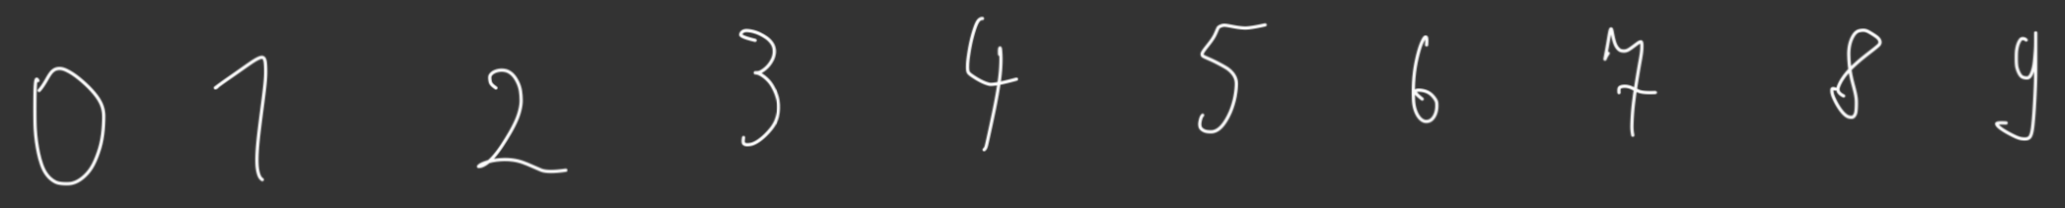
\includegraphics[width=\textwidth]{digits.png}
\caption{Pierwszy zestaw odręcznie zapisanych cyfr.}
\end{figure}

\subsection{Wyniki testowe na własnym zbiorze}
Sieć osiągnęła dokładność na poziomie \textbf{83.33\%}. Szczegółowe wyniki dla poszczególnych cyfr przedstawiono poniżej:
\begin{itemize}
    \item \textbf{Cyfry rozpoznane poprawnie w 100\%}: 0, 1, 2, 3, 4, 5, 8.
    \item \textbf{Cyfry z błędami}:
    \begin{itemize}
        \item 6: \textit{dwa razy pomylona z 8}
        \item 7: \textit{raz pomylona z 1}
        \item 9: \textit{dwa razy pomylona z 4}
    \end{itemize}
\end{itemize}

\subsection{Analiza błędów}
Błędy w rozpoznawaniu mogą wynikać z:
\begin{itemize}
    \item Słabego odróżniania podobnych cyfr (np. 4 i 9, 6 i 8).
    \item Indywidualnych cech pisma ręcznego użytkownika.
    \item Braku zróżnicowania treningowego zbioru danych.
    \item Faktu, że EMNIST, to amerykański zbiór, a Amerykanie zapisują cyfry w trochę inny sposób niż Polacy.
\end{itemize}

\section{Zadanie 3}
\subsection{Polecenie}
Korzystając z jednej z dostępnych bibliotek stwórz i wytrenuj klasyfikator oparty o \textit{Random Forest}
rozpoznającą cyfry z podanego zbioru danych. Jaki współczynnik prawidłowej
rozpoznawalności ma ten klasyfikator na zbiorze testowym? Jaka jest czułość i precyzja?

\subsection{Opis modelu}
Do klasyfikacji cyfr wykorzystano model Random Forest dostępny w bibliotece \texttt{scikit-learn}.
Algorytm Random Forest, to jeden z najpopularniejszych klasyfikatorów opartych na drzewach decyzyjnych. Random Forest buduje wiele drzew decyzyjnych na różnych próbkach treningowych i używa większościowego głosowania do klasyfikacji. Dane wejściowe zostały spłaszczone do postaci wektora o wymiarze 784 (28x28 pikseli), co jest standardową metodą przygotowania danych do klasyfikacji z użyciem algorytmu Random Forest.

\subsection{Wyniki testowe}
Klasyfikator został przetestowany na zbiorze MNIST, osiągając następujące wyniki:
\begin{itemize}
    \item Dokładność: \textbf{97.04\%}
    \item Precyzja: \textbf{97.03\%}
    \item Czułość: \textbf{97.01\%}
\end{itemize}

\begin{table}[H]
\centering
\begin{tabular}{|c|c|c|c|c|}
\hline
\textbf{Cyfra} & \textbf{Precyzja} & \textbf{Czułość} & \textbf{F1-score} & \textbf{Liczba egzemplarzy} \\ \hline
0              & 0.9681            & 0.9908           & 0.9793            & 980                    \\ \hline
1              & 0.9877            & 0.9930           & 0.9903            & 1135                   \\ \hline
2              & 0.9616            & 0.9709           & 0.9662            & 1032                   \\ \hline
3              & 0.9633            & 0.9624           & 0.9629            & 1010                   \\ \hline
4              & 0.9745            & 0.9725           & 0.9735            & 982                    \\ \hline
5              & 0.9762            & 0.9641           & 0.9701            & 892                    \\ \hline
6              & 0.9760            & 0.9781           & 0.9771            & 958                    \\ \hline
7              & 0.9715            & 0.9621           & 0.9668            & 1028                   \\ \hline
8              & 0.9617            & 0.9548           & 0.9583            & 974                    \\ \hline
9              & 0.9620            & 0.9524           & 0.9572            & 1009                   \\ \hline
\textbf{Średnia}  & \textbf{0.9703}   & \textbf{0.9701}  & \textbf{0.9702}   & 10000                  \\ \hline
\end{tabular}
\caption{Szczegółowe wyniki klasyfikacji dla Random Forest na zbiorze MNIST.}
\end{table}

\subsection{Porównanie wyników}
\begin{figure}[H]
\centering
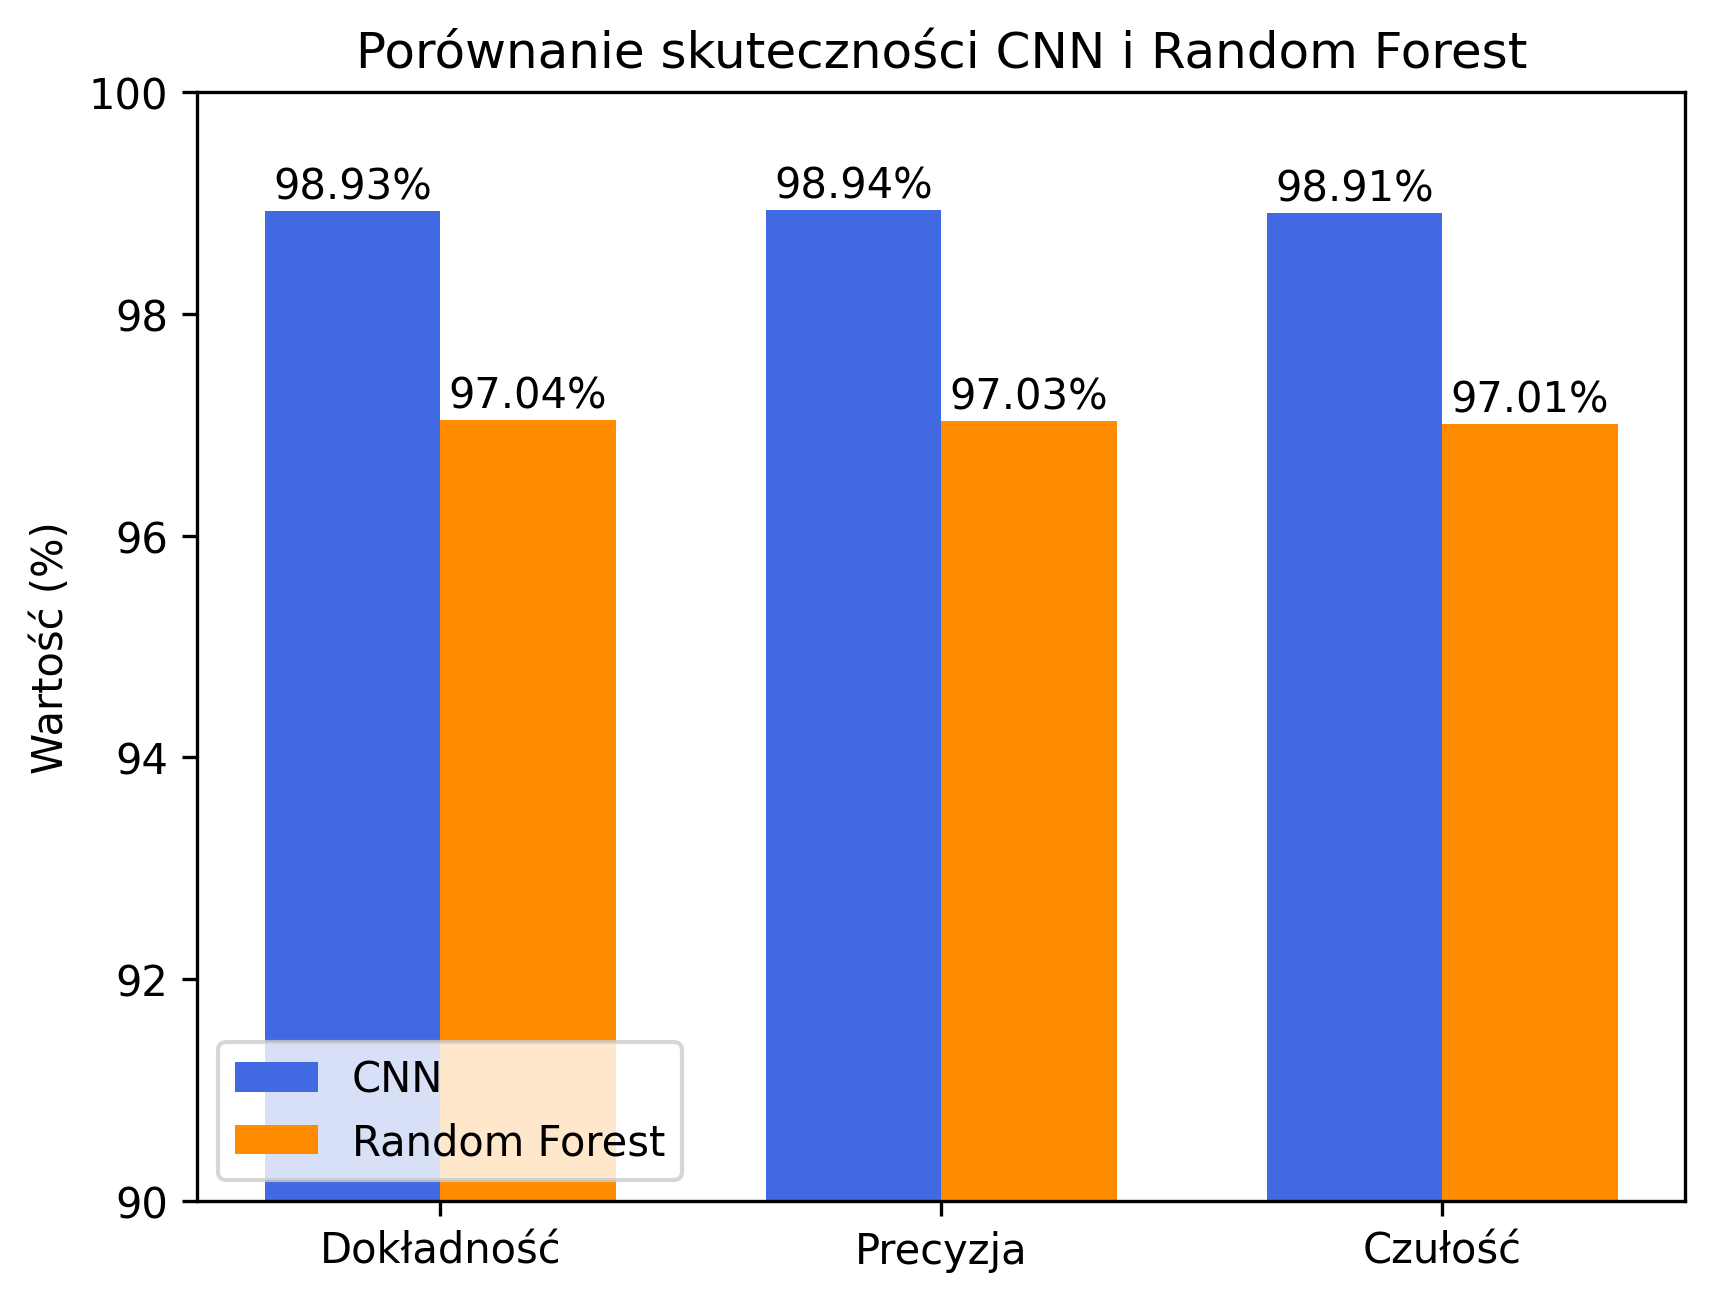
\includegraphics[width=\textwidth]{performanceComparison.png}
\caption{Porównanie skuteczności CNN i Random Forest.}
\end{figure}

W porównaniu do sieci neuronowej, klasyfikator Random Forest osiągnął nieco gorsze wyniki. Może to wynikać z faktu, że modele oparte na drzewach decyzyjnych nie są tak skuteczne w analizie obrazów jak głębokie sieci neuronowe, które lepiej radzą sobie z wykrywaniem złożonych wzorców wizualnych. Niemniej jednak, Random Forest pozostaje efektywną alternatywą w przypadku ograniczonych zasobów obliczeniowych, ponieważ nie wymaga tak dużej ilości danych treningowych ani intensywnego przetwarzania jak głębokie sieci neuronowe.

\section{Podsumowanie}
Sieć neuronowa wykazała bardzo wysoką skuteczność na zbiorze MNIST, jednak jej skuteczność na zbiorze własnych próbek była zauważalnie niższa. Klasyfikator Random Forest osiągnął nieco gorsze wyniki na MNIST, ale nadal prezentował wysoką skuteczność. Aby poprawić dokładność na niestandardowych próbkach, można by:
\begin{itemize}
    \item \textbf{Powiększenie zbioru danych treningowych}: Zwiększenie liczby próbek w zbiorze treningowym, szczególnie poprzez dodanie bardziej zróżnicowanych przykładów pisma odręcznego (np. od różnych osób, w różnych stylach), mogłoby pomóc modelowi lepiej generalizować.
    \item \textbf{Zastosowanie metod augmentacji danych}: Techniki takie jak obrót, skalowanie, przesunięcie czy dodanie szumu do obrazów mogą sztucznie zwiększyć różnorodność zbioru treningowego. Na przykład, obrót o kilka stopni lub zmiana grubości linii w cyfrach mogłaby lepiej przygotować model na różnice w indywidualnym piśmie.
    \item \textbf{Dostosowanie architektury modelu}: W przypadku sieci neuronowej można rozważyć dodanie większej liczby warstw konwolucyjnych lub zwiększenie liczby filtrów, aby model mógł wychwycić bardziej subtelne cechy pisma. Dla Random Forest można by zwiększyć liczbę drzew decyzyjnych lub dostosować parametry, takie jak maksymalna głębokość drzew, aby lepiej radzić sobie z różnorodnością danych.
\end{itemize}

\end{document}
